\documentclass[12pt,a4paper]{article}
% Estilo compartido para informes. Compilar con LuaLaTeX desde tp1/.
\usepackage[spanish,es-nodecimaldot]{babel}
\usepackage{fontspec}
\setmainfont{Montserrat-Medium.ttf}[
  Path=../assets/fonts/,
  BoldFont=Montserrat-Bold.ttf,
  ItalicFont=Montserrat-MediumItalic.ttf]
\usepackage[a4paper,margin=2.5cm,headheight=16pt]{geometry}
\usepackage{xcolor,graphicx,booktabs,tabularx}
\usepackage{float}
\usepackage{titlesec,fancyhdr,enumitem,caption}
\usepackage{ragged2e}
\usepackage{hyperref}
\definecolor{verde}{HTML}{1D4036}
\definecolor{bronce}{HTML}{D38129}
\definecolor{rosa}{HTML}{D88E77}
\definecolor{calido}{HTML}{EFE4D8}
\definecolor{grafito}{HTML}{1D1D1D}
\hypersetup{colorlinks=true,linkcolor=verde,urlcolor=verde,
  pdftitle={TP1 - Instalación de máquinas virtuales},pdfsubject={Cyberseguridad}}
\AtBeginDocument{\color{grafito}\RaggedRight\fontsize{12}{14.4}\selectfont}
\setlength{\parindent}{0pt}
\setlength{\parskip}{7pt}
\setlist[itemize]{leftmargin=*,itemsep=7pt,topsep=4pt}
\setlist[enumerate]{leftmargin=*,itemsep=6pt}
\titleformat{\section}{\color{verde}\bfseries\fontsize{18}{21.6}\selectfont}{\thesection}{0.65em}{}
\titleformat{\subsection}{\color{verde}\bfseries\large}{\thesubsection}{0.65em}{}
\titleformat{\subsubsection}{\color{verde}\bfseries}{\thesubsubsection}{0.65em}{}
\titlespacing*{\section}{0pt}{16pt}{8pt}
\titlespacing*{\subsection}{0pt}{12pt}{5pt}
\titlespacing*{\subsubsection}{0pt}{10pt}{4pt}
\setcounter{tocdepth}{2}
\pagestyle{fancy}
\fancyhf{}
\fancyhead[L]{\small\color{verde}FCEFyN | UNC}
\fancyhead[R]{\small\color{verde}\materia\ · TP \numeroTP}
\fancyfoot[L]{\scriptsize Informe de laboratorio}
\fancyfoot[R]{\small\thepage}
\renewcommand{\headrulewidth}{0.4pt}
\captionsetup{font=small,labelfont=bf,justification=raggedright,singlelinecheck=false,hypcap=false}
\newcommand{\pendiente}[1]{\par{\small\color{verde}\textbf{Por completar.} #1\par}}
% Si falta una captura se muestra un espacio reservado; no impide compilar.
\newcommand{\captura}[2]{%
  \par\smallskip\begingroup\centering
  \IfFileExists{figuras/#1}{%
    \includegraphics[width=\linewidth,height=5cm,keepaspectratio]{figuras/#1}%
  }{%
    \setlength{\fboxsep}{10pt}%
    \fcolorbox{bronce}{calido}{\parbox[c][1.25cm][c]{\dimexpr\linewidth-2\fboxsep-2\fboxrule\relax}{%
      \centering\small Captura pendiente\par\texttt{\detokenize{#1}}}}%
  }%
  \captionof{figure}{#2}\par\endgroup\smallskip
}

\usepackage{xurl}

\newcommand{\materia}{Cyberseguridad}
\newcommand{\numeroTP}{5}
\newcommand{\tituloTP}{Captura DNS sobre UDP}
\newcommand{\estudiante}{Brigido Tomas Andres}
\newcommand{\legajo}{38481096}
\newcommand{\carrera}{ICOMP}
\newcommand{\docente}{Javier A. Jorge}


% Metadatos específicos del TP5 y capturas en img/.
\hypersetup{pdftitle={TP5 - Captura DNS sobre UDP}}
\renewcommand{\captura}[2]{%
  \begin{figure}[H]
    \centering
    \IfFileExists{img/udp/#1}{%
      \includegraphics[width=0.85\linewidth,height=5cm,keepaspectratio]{img/udp/#1}%
    }{%
      \setlength{\fboxsep}{10pt}%
      \fcolorbox{bronce}{calido}{\parbox[c][1.1cm][c]{0.85\linewidth}{%
        \centering\small Captura pendiente\par\texttt{\detokenize{#1}}}}%
    }%
    \caption{#2}
  \end{figure}
}

\begin{document}
\hypersetup{pageanchor=false}
\begin{titlepage}
  
\includegraphics[width=8cm]{../assets/logo-fcefyn-2026.png}
  \vspace{1cm}

  {\color{verde}\small UNIVERSIDAD NACIONAL DE CÓRDOBA\par}
  \vspace{2.1cm}
  {\color{bronce}\bfseries\large TRABAJO PRÁCTICO \numeroTP\par}
  \vspace{0.45cm}
  {\color{verde}\bfseries\fontsize{32}{38.4}\selectfont Captura DNS\\sobre UDP\par}
  \vspace{0.3cm}
{\small Actividades 10.2.7 y 17.1.7\par}
\vspace{0.35cm}
  {\large \materia\par}
  \vspace{0.8cm}
  {\color{bronce}\rule{2.7cm}{2pt}\par}
  \vfill
  \renewcommand{\arraystretch}{1.45}
  \begin{tabular}{@{}p{3.2cm}p{10cm}@{}}
    Estudiante & \estudiante \\
    Legajo & \legajo \\
    Carrera & \carrera \\
    Docente & \docente \\
  \end{tabular}
  \vfill
  {\small Córdoba, Argentina\par}
\end{titlepage}
\hypersetup{pageanchor=true}

\tableofcontents
\vspace{1cm}
\newpage

\section{Introducción y objetivos}
Esta actividad analiza consultas y respuestas DNS mediante Wireshark. Se registra la configuración de la VM y se examinan los campos de Ethernet, IPv4 y UDP.

\section{Parte 1: configuración IP}
\begin{verbatim}
ifconfig
cat /etc/resolv.conf
netstat -rn
\end{verbatim}
\begingroup
\small\renewcommand{\arraystretch}{1.4}
\begin{tabularx}{\linewidth}{@{}>{\RaggedRight\arraybackslash}p{6cm}X@{}}
\toprule
\textbf{Descripción} & \textbf{Resultado} \\
\midrule
Dirección IP & 192.168.1.3 \\
Dirección MAC & d8:5e:d3:53:a1:c0 \\
Dirección IP del gateway predeterminado & 192.168.1.1 \\
Dirección IP del servidor DNS & 192.168.1.1 \\
\bottomrule
\end{tabularx}
\endgroup

\section{Parte 3: análisis de los paquetes}
\subsection{Consulta DNS}

\begin{figure}[H]
    \centering
    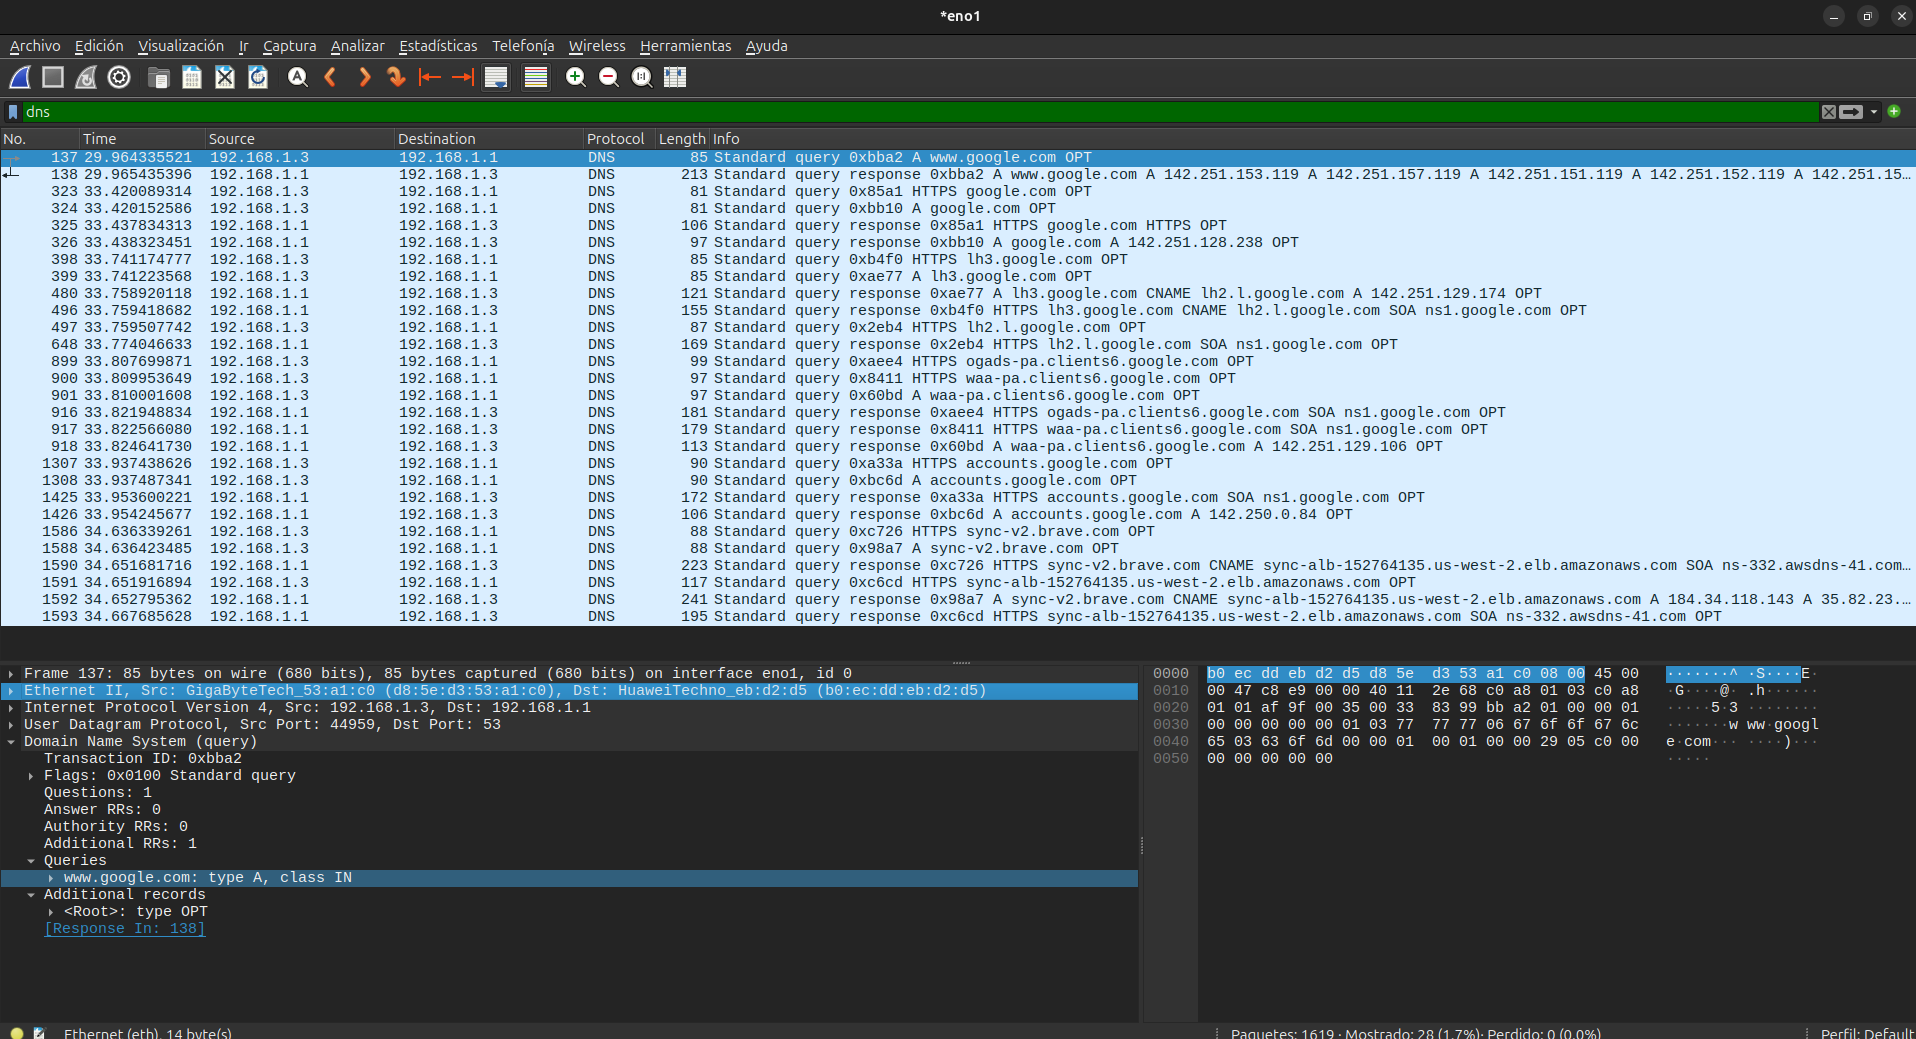
\includegraphics[width=0.9\textwidth]{img/udp/maciguales.png}
    \caption{Campos de la consulta DNS seleccionada.}
    \label{fig:captura-dns}
\end{figure}

\par\textbf{¿Es la dirección MAC de origen la misma que la registrada en la Parte 1 para la VM?}

Si, es la misma dirección MAC de origen que la registrada en la Parte 1.

\par\textbf{¿Puede identificar la dirección IP y dirección MAC de origen y destino de este paquete?}

\begingroup
\small\renewcommand{\arraystretch}{1.4}
\begin{tabularx}{\linewidth}{@{}>{\RaggedRight\arraybackslash}p{6cm}X@{}}
\toprule
\textbf{Descripción} & \textbf{Resultado} \\
\midrule
IP del cliente & 192.168.1.3 \\
MAC del cliente & d8:5e:d3:53:a1:c0 \\
IP de destino & 192.168.1.1 \\
MAC de destino & b0:ec:dd:eb:d2:d5 \\
\bottomrule
\end{tabularx}
\endgroup

\begin{figure}[H]
    \centering
    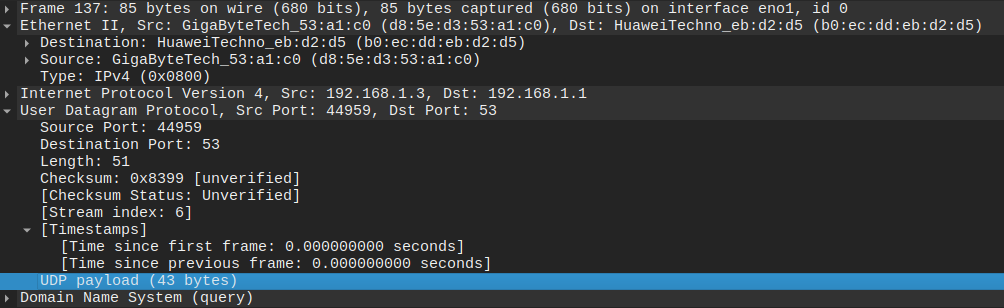
\includegraphics[width=0.9\textwidth]{img/udp/udp.png}
    \caption{Campos UDP de la consulta DNS.}
    \label{fig:captura-dns}
\end{figure}

\subsection{Campos UDP y comparación con la configuración}

\begin{figure}[H]
    \centering
    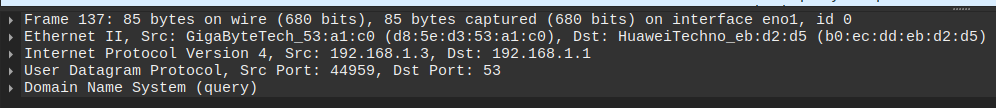
\includegraphics[width=0.9\textwidth]{img/udp/information.png}
    \caption{Campos de información UDP.}
    \label{fig:captura-dns}
\end{figure}

\begingroup
\small\renewcommand{\arraystretch}{1.4}
\begin{tabularx}{\linewidth}{@{}>{\RaggedRight\arraybackslash}p{6cm}X@{}}
\toprule
\textbf{Descripción} & \textbf{Resultado} \\
\midrule
Tamaño de la trama & 85 \\
Dirección MAC de origen & d8:5e:d3:53:a1:c0 \\
Dirección MAC de destino & b0:ec:dd:eb:d2:d5 \\
Dirección IP de origen & 192.168.1.3 \\
Dirección IP de destino & 192.168.1.1 \\
Puerto de origen & 44959 \\
Puerto de destino & 53 \\
\bottomrule
\end{tabularx}
\endgroup

\pendiente{Registrar también la longitud y el checksum de UDP e identificar su encabezado y los datos DNS.}
\par\textbf{¿Es la dirección IP de origen la misma que la dirección IP de la PC local que registró en la parte 1?}

Si, es la misma dirección IP de origen que la registrada en la Parte 1.

\par\textbf{¿Es la dirección IP de destino la misma que la puerta de enlace predeterminada (gateway) que observó en la parte 1?}

Si, es la misma dirección IP de destino que la puerta de enlace predeterminada (gateway) que se observó en la Parte 1.


\subsection{Respuesta DNS}

\begin{figure}[H]
    \centering
    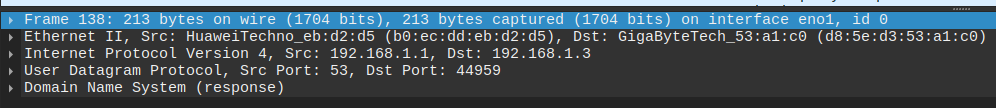
\includegraphics[width=0.9\textwidth]{img/udp/respuesta.png}
    \caption{Campos de la respuesta DNS y direcciones resueltas.}
    \label{fig:captura-dns}
\end{figure}

\par\textbf{En la trama Ethernet II para la respuesta de DNS, ¿qué dispositivo es la dirección MAC de origen y qué dispositivo es la dirección MAC de destino?}
Origen: el router (\texttt{b0:ec:dd:eb:d2:d5}). Destino: la PC local (\texttt{d8:5e:d3:53:a1:c0}).

\par\textbf{¿Cuál es la dirección IP de destino?}
\texttt{192.168.1.3}, la PC local.

\par\textbf{¿Cuál es la dirección IP de origen?}
\texttt{192.168.1.1}, el router que actúa como servidor DNS.

\par\textbf{¿Qué sucedió con los roles de origen y destino correspondientes a la VM y al gateway predeterminado?}
Se invirtieron: el router envía la respuesta y la PC local la recibe.

\section{Reflexión}
\par\textbf{¿Cuáles son los beneficios de utilizar UDP en lugar de TCP como protocolo de transporte para DNS?}

UDP no necesita establecer una conexión y tiene un encabezado más pequeño, lo que reduce la demora y el tráfico en consultas DNS simples.

\par\textbf{A partir de los resultados de Wireshark. ¿qué más podemos averiguar sobre la red si quitamos el filtro?}

Podemos observar otros protocolos, direcciones, puertos y comunicaciones presentes en la captura.

\par\textbf{¿De qué manera un atacante puede utilizar Wireshark para poner en riesgo la seguridad de sus redes?}

Puede analizar el tráfico al que tenga acceso para identificar equipos y servicios, y obtener datos sensibles si se transmiten sin cifrar.

\newpage
\section{Referencias}
Cisco Networking Academy. \textit{Utilizar Wireshark para examinar una captura DNS de UDP}, 2017--2020. Consigna: \textit{10.2.7 Lab - Using Wireshark to Examine a UDP DNS Capture.pdf}.
\par Cisco Networking Academy. \textit{Explorar tráfico DNS}, 2017--2020. Consigna: \textit{17.1.7 Lab - Exploring DNS Traffic.pdf}.
\end{document}
